%!TEX root = ../../Master.tex
\section{Leading Technologies}

http://www.wifarer.com/hospitals
http://www.meridianapps.com/products
http://www.smartindoor.com/
https://www.indooratlas.com/
http://theory.stanford.edu/~amitp/GameProgramming/Heuristics.html

\subsection{Position Technologies}

  \subsection{Satellites}

  \subsection{Cellular Communication Network}

  \subsection{Infra-red}

  \subsection{Blue-tooth}

  \subsection{WIFI}

  \subsection{Summary of Position Technologies}

\subsection{Positioning Techniques}

  \subsection{Cell of Origin}

  \subsection{Angle of Arrival}

  \subsection{Angle difference of Arrival}

  \subsection{Time of Arrival}

  \subsection{Time difference of Arrival}

  \subsection{Triangulation}

  Triangulation is a method used for estimating the position of an object. The method uses the properties of triangles. Triangulation has two derivatives: literation and angulation.

 \subsubsection{Lateration}

  Lateration is commonly used technique for positioning.  Lateration uses the distance between known locations and and the point to be determined, to estimate the location.\cite{tri_lateration}  There are two types of lateration two dimensional and three dimensional. The two dimensional are use in robots that navigates in only one plane, like robot vacuum cleaners. 
  lateration in three dimensions are used in GPS positioning, and other practical applications for positioning.
  We will only explain three dimensional lateration.
  \begin{figure}[ht!]
  \centering
  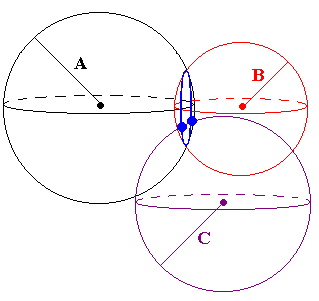
\includegraphics[width=3in]{trilateration}
  \caption{Example of lateration with three know positions.}
  \label{fig:trilateration}
  \end{figure}
  

  Trilateration in three dimensions is possible in fare most situations if and only if the distance to three known positions is defined or possible to calculate.
  If we know a distance to one of these three positions we know that the point we are seeking is in the surface of a sphere, with center at the know position, and with a radius equals to the distance to the center. This is illustrated on \cref{fig:trilateration} as the surface of the sphere A.

  The intersection of two spheres is a circle. By determining the distance to a second know point it is possible to circumscribe the range of possible position to a smaller area.
  This is illustrated as the blue circle on \cref{fig:trilateration}, and is the intersection between sphere A and B.
  A third sphere that overlaps the intersection between the first two spheres, will mark 2 points where all three spheres is collapsing. In fare most situations there are only one of these locations that lies on the Earth's surface, the other point will often be fare in to the sky or deep inside earth. So by sorting one point from, there is only one possible position left. 
  In some very rare situation it is possible that both point lies on the Earth's surface, and in such situations the use of four spheres will determine witch of the to positions is the right one.



  \subsubsection{Angulation}

  Angulation uses the technique called Angle of Arrival (AOA), which can compute the location of a source. The parameters needed are as minimum two relative angles between a remote point and the source, and the distance between the remote points. The source is at the location where the lines formed by the angle direction lines intercept. 

  In 2D, as few as two remote points are needed, given the source is not directly in between the remote points. However to improve accuracy and remove ambiguity  another remote point is needed. In 3D, as few as three remote points are needed. However as with 2D, another remote point improves accuracy and removes ambiguity. \cite{Liu2007, Sun2009, Boontrai2009}

  For example, rangers in location known fire lookout towers can use AOA to pinpoint where the fire is. See \cref{fig:aoa} A ranger at tower A sees the fire and notates the bearing to the fire. He then communicates with a ranger at tower B telling him the general direction of the fire. The ranger at tower B now notates the bearing to the fire from his perspective. The fire can now be pinpointed from the 2 remote points (given the fire started in a 2-D world). The fire is where the 2 angle direction lines intercept A ranger at tower C can verify this position by also noting his bearing. \cite{compassdude_triangulation}

  \begin{figure}
    \centering
    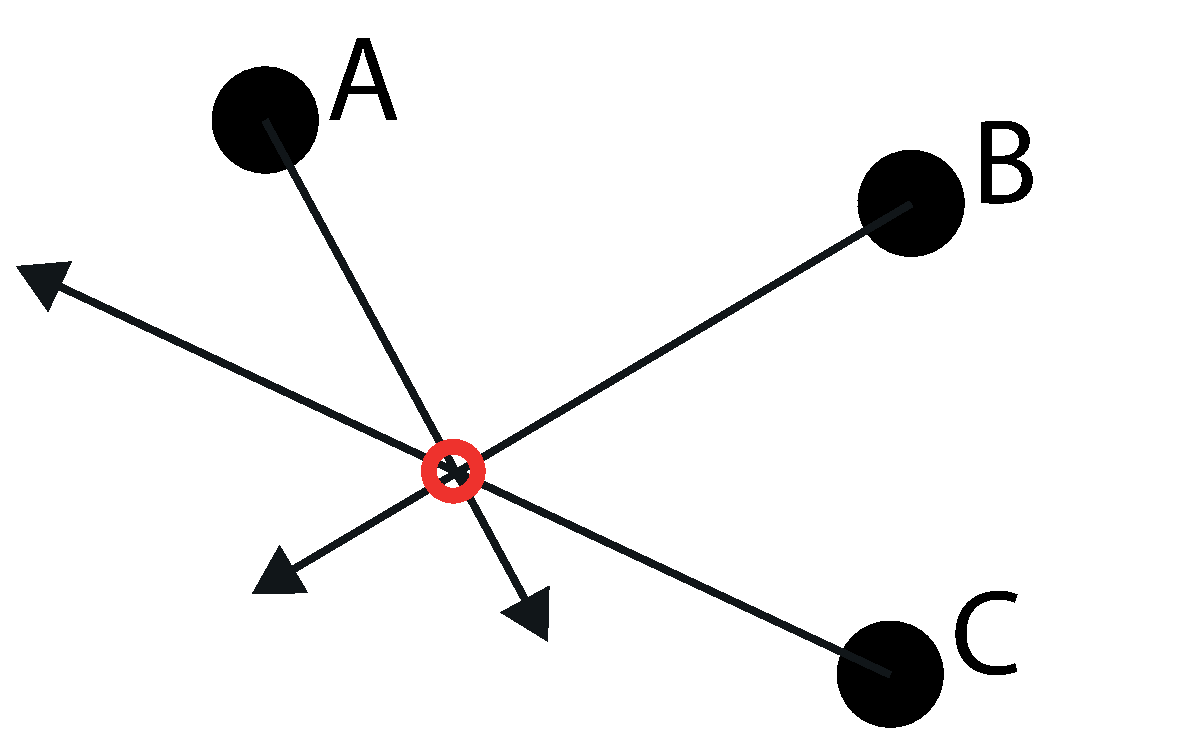
\includegraphics[width=\textwidth]{aoa.eps}
    \caption{Example of fire lookout towers positioning a fire using AOA.}
      \label{fig:aoa}
  \end{figure}

  The advantages of AOA are the few remote points needed in order to estimate a position. Another advantage is the independency of time synchronization.

  The disadvantages of AOA are the need of large and complex hardware requirements, and degradation of the location estimate as the target moves away from the measuring units. In order to perform accurate position of the target, very accurate angle measurements need to be performed. This can become a problem if the measuring is done in wireless networks, because of shadowing, multipath reflections arriving from misleading directions etc. Therefore angulation is best performed in free space.

  \subsection{Location Fingerprinting}

  Location fingerprinting refers to the algorithms that first collect characteristics (fingerprints) of a scene and then matches these a priori characteristics with the characteristics of the location the source is in, to determine the source' location.

  There are two stages for location fingerprinting. The offline state where a site survey is performed in the environment. The characteristics of known locations are stored in databases. In the online state, these a priori characteristics are used to match the location of the source.

  The main challenge of location fingerprinting is the possibility of variating signal strengths corrupting characteristics data.

  Some of the existing location fingerprinting-based positioning algorithms will be described below.

  \subsubsection{k-nearest-neighbour}

  The k-nearest-neighbour (k-NN) algorithm simply compares a data set to $k$ closest-neighbour data sets, meaning data sets that are close to the original data set. The closeness is called the distance and is typically computed using the Euclidean distance or the Hamming distance.\cite{Liu2007, wiki_knn}

  In location fingerprinting, k-NN uses the online Received Signal Strengths (RSS) to find the closest $k$ locations from the a priori RSS.


  \subsection{Summary of Position Techniques}

  \subsection{Information Techniques}

  \subsubsection{2 Dimensional map}

  \subsubsection{3 Dimensional map}

  \subsubsection{Text directions}

  \subsubsection{Summary of Information Techniques}

\newpage

\subsection{Path finding Algorithms}

  Path finding algorithms are used for finding a path between two locations, the source and the destination. By searching its way from the source to the destination, until a path is found. These algorithms also make it possible to calculate the optimal path, i.e. the shortest.

  The algorithms to perform searches make use of a weighted graph. A graph, $G$ is a set of nodes $V$, connected by links $E$.
  Information about destinations, rooms, entrances and exits would be represented as nodes and hallways and stairs would be represented as links. The distance to travel from node to node via a particular link, would be represented as a weight $W(e)$.

  \begin{figure}[ht!]
    \centering
    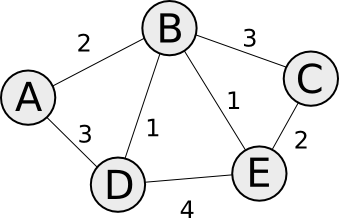
\includegraphics[width=\textwidth]{Graph}
    \caption{A Graph}
    \label{overflow}
  \end{figure}

  An important factor of a searching algorithm is correctness and also the time required to calculate the optimized path.
  The algorithms can be rated by their worst-case time, to ensure a responsive performance.

  \subsubsection{Dijkstra's Algorithm}

  A commonly used algorithm for finding the shortest path is Dijkstra's algorithm. It loops through steps until all nodes to the target node is optimized with the least cost, then points out the shortest path from source node, to target node. Because of the need of every node being evaluated, the complexity of algorithm is proportional to the number of nodes, which means that a lot of computational power is required to calculate the result. \sinote{Vis kompleksitet med store O notation?} \cite{Dijkstra}

  \begin{figure}[ht!]
    \centering
    \frame{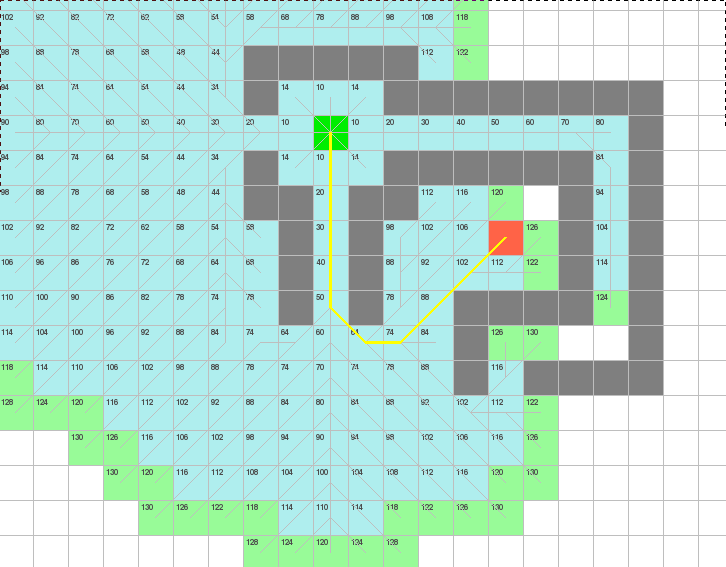
\includegraphics[width=\textwidth]{Dijkstra}}
    \caption{Dijkstra's algorithm in action}
    \label{overflow}
  \end{figure}

  We consider the problem: find shortest path from source to target.

  Where $P$ is the source node, $Q$ is the target and $R$ is the evaluating node.

  The nodes are subdivided into three sets:

\sinote{Forslår description environment her. Skaber mere overblik}
  Set $A$ - Optimized nodes (least costly path from $P$ is known)
  Set $B$ - Temporary nodes (evaluated cost of path from $P$ but not part of set $A$)
  Set $C$ - Remaining nodes

  The links are subdivided into three other sets:

\sinote{Forslår description environment her. Skaber mere overblik}
  Set \RN{1} - Links used in the set $A$
  Set \RN{2} - Not part of set I (one and only one link of this set will lead to each node in set $B$)
  Set \RN{3} - Remaining links (rejected or not yet considered)

  At first all nodes is assigned to set $C$ and all links to set \RN{3}, P is then assigned to set $A$.
  Then we loop through following steps until $Q$ is part of set $A$.

\sinote{Forslår description environment her. Skaber mere overblik}
  Step 1. Consider all the links r connecting the node just assigned to set $A$. If $R$ is part of set $C$ assign to set $B$ and assign r to set \RN{2}. \sinote{simon: R eller r?}
  If R is part of set $B$, then investigate if the use of link r is less costly from $P$ to R than the existing link in set \RN{2}. If less costly assign link r and reject existing link in set \RN{2}, otherwise reject r to set \RN{3}.

  Step 2. For each node in set $B$ where there is only one path in set \RN{1} and set \RN{2}, the node with minimum cost from $P$ is assign to set $A$ and with the corresponding link assign to set \RN{1}.

  \begin{figure}[ht!]
    \centering
    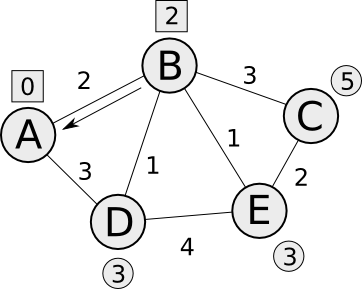
\includegraphics[width=\textwidth/3]{DijkstraX}
    \caption{Dijkstra calculation}
    \label{overflow}
  \end{figure}

  \subsubsection{Best-First-Search}

  Best-First-Search is search algorithm like Dijkstra's algorithm, with the exception that is uses heuristic to estimate how far target the node is the an evaluating node, then it repeatedly choose the node with the least cost, until target node is reached. \sinote{nok bedst du selv lige læser denne sætning igennem igen. Skal måske omformuleres} The final path is not guaranteed the shortest, however it it not as complex as Dijkstra's algorithm which means it is much faster to calculate. \cite{BestFirst}

  But when obstacles are introduced, like walls, the Best-First-Search algorithm fails to find a path that is close to optimal.

  \begin{figure}[ht!]
    \centering
    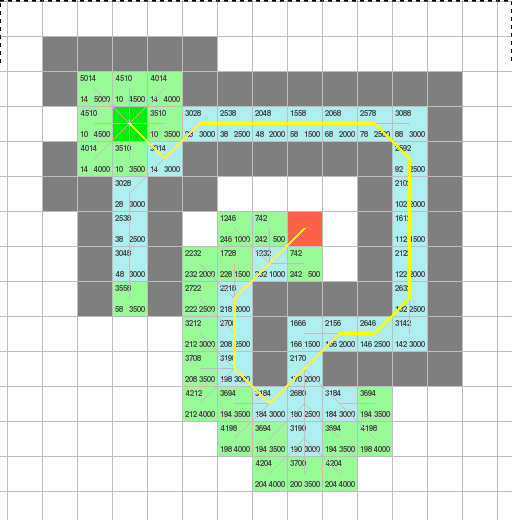
\includegraphics[width=\textwidth]{BestFirst} 
    \caption{Best-First-Search in action}
    \label{bestfirst}
  \end{figure}

  \subsubsection{A* Algorithm}

  If you would combine Dijkstra's algorithm with Best-First-Search algorithm, you would get the A* algorithm which also utilises the principle of a heuristic estimation to determine which node to test next. It uses a evaluation function $f(x) = g(x) + h(x)$, where $g(x)$ describes the cost from the start to the node being evaluated, and $h(x)$ is a heuristic function that estimates the cost from the evaluating node to the target node. \cite{http://theory.stanford.edu/}

\sinote{brug evt itemize}
  - If $h(x)$ is zero, then only $g$ affects the result and making it work like Dijkstra's algorithm.

  - If $h(x) < g(x)$, the algorithm will guaranteed find the shortest path from source to target, at a slow running time.

  - If $h(x) == g(x)$ \sinote{bare = i stedet for ==?}, the algorithm will only extract the best path, but this not always possible due to obstacles.

  - If $h(x) > g(x)$, the algorithm will find a path fast not its not always the optimal, then works like the Best-First-Search algorithm.\sinote{skal måske omformuleres?}

  This means that the heuristic estimation should be reasonable, $h(x)$ should be admissible and not overestimate the distance between the evaluating node and the target node. But should be just right for the final chosen path to be the optimal path and the for the complexity of the algorithm to be at a minimum. Each step the algorithm evaluates the value of $f(x)$ of each node to pick the next node with the smallest cost.

  \begin{figure}[ht!]
    \centering
    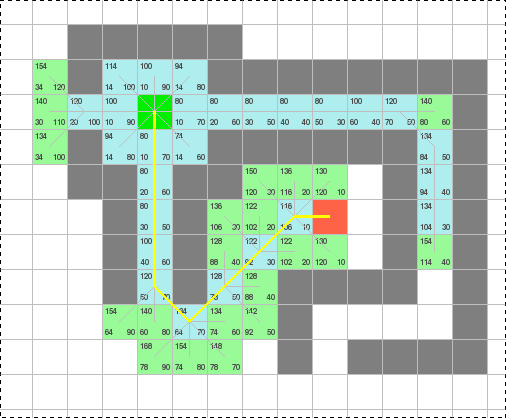
\includegraphics[width=\textwidth]{AstarHlow}
    \caption{A* algorithm with an admissible heuristic value}
    \label{astar}
  \end{figure}

  There is multiple ways to calculate the heuristic value(estimated cost) to the target node, but an ideal choice would be the Euclidean \ref{equation:Euclidean} \sinote{brug evt. cref i stedet. Den indsætter selv eq. og nummer.} distance, as no path can be shorter than the direct distance between two nodes.
  \begin{equation} \label{equation:Euclidean}
    dist((x, y), (a, b)) = \sqrt{(x - a)^2 + (y - b)^2}
  \end{equation}

  \subsubsection{Summary of Algorithms}

  Path algorithms searches for a path to target. Some focuses on finding a path fast, others finding the most optimal path. Using the A* algorithm with a heuristic model that is admissible, which underestimates the cost to the target path, assure an optimal path without calculating every node. See \cref{tbl:scheme}
  
  \begin{table}[ht!]
    \centering
  \rowcolors{1}{}{lightgray}
    \begin{tabular}{|r|l|c|}
      \hline
      \textbf{Algorithm} & \textbf{Advantages} & \textbf{Disadvantages} \\
      \hline
      Dijkstra's & Always optimal path & Slow calculation \\
      Best-First-Search & Fast calculation & Not always optimal path \\
      A* & Optimal path if $h(x)<g(x)$, Fast calculation & Not always optimal path \\
      \hline
    \end{tabular}
    \caption{Table of advantages/disadvantages of different algorithms}
    \label{tbl:scheme}
  \end{table}